\subsection{Thiết kế bảng khảo sát}
% Giới thiệu survey %
Đánh giá \emph{external quality} đồng nghĩa với việc đánh giá được sự hài lòng của người dùng hoặc khách hàng đối với một quy trình nghiệp vụ. Để làm được như vậy, cần phải thu thập những ý kiến của người sử dụng hoặc theo dõi và tự động đánh giá quá trình người dùng thực thi quy trình nghiệp vụ. Ngày nay, có một số công cụ dưới dạng các ứng dụng mở rộng (add-on extensions) trên các trình duyệt web, cho phép tích hợp vào hệ thống để theo dõi các luồng thực thi của khách hàng trên một quy trình cụ thể, chẳng hạn như khách hàng có hoàn thành phiên hoạt động của mình hay không, khách hàng có rơi vào những trường hợp ngoại lệ không, có khách hàng nào dừng quy trình giữa chừng hay không.
Ứng dụng các công cụ trên vào đánh giá chất lượng bên ngoài của quy trình có thể đảm bảo tính chính xác, và được thực thi một cách tự động dựa trên việc theo dõi hành vi của người dùng, không tốn nhiều thời gian, công sức của người dùng . Tuy nhiên, không phải quy trình nghiệp vụ nào cũng có thể được tích hợp công cụ trên. Một số quy trình nghiệp vụ cần được thực thi ngoài thực tế, không phải trên các trang web hay hệ thống máy tính, dẫn tới không thể ứng dụng các công cụ theo dõi hành vi người dùng vào những quy trình nghiệp vụ này. Chúng tôi nhận thấy rằng, đối với những loại quy trình này nói riêng, hay cả những quy trình khác nói chung, đều có thể thu thập được sự hài lòng và trải nghiệm của người dùng thông qua các cuộc khảo sát (survey).
\par
Khảo sát đã được ứng dụng từ lâu để lấy ý kiến khách hàng về một dịch vụ, sản phẩm,... hay thậm chí là cả một tổ chức, một doanh nghiệp. Ngày nay, khảo sát vẫn là một công cụ phổ biến và hiệu quả để thu thập thông tin từ người dùng, cho nên ta có thể sử dụng khảo sát, với các câu hỏi khai thác hợp lý, có thể đánh giá được thái độ của khách hàng đối với quy trình nghiệp vụ cụ thể như thế nào, từ đó có thể rút ra được \emph{external quality} của quy trình. Khảo sát có thể được thực thi trên nhiều nền tảng khác nhau với nhiều hình thức khác nhau, chẳng hạn như có thể khảo sát khách hàng thông qua chatbot - là một phần mềm ứng dụng trí tuệ nhân tạo để mô phỏng lại các cuộc trò chuyện với người dùng, thông qua cuộc trò chuyện đó có thể lấy được thông tin từ người dùng. Hoặc có thể là một bảng khảo sát trực tuyến với các câu hỏi đa dạng hình thức được thiết kế sẵn để người dùng trả lời và gửi phản hồi về quy trình đó. Khảo sát trực tuyến có một số lợi ích như sau:
\begin{itemize}
    \item Người dùng có thể thực hiện khảo sát bất cứ khi nào họ muốn.
    \item Người dùng có thể dành nhiều thời gian hơn để trả lời các câu hỏi, nói cách khác, họ không bị ràng buộc thời gian.
    \item Khảo sát trực tuyến cho phép người thiết kế đưa ra nhiều hình thức câu hỏi khác nhau để đánh giá nhiều khía cạnh khác nhau của vấn đề cần được khảo sát (câu hỏi hai đáp án, nhiều đáp án, câu hỏi dạng thang điểm,...).
\end{itemize}
\par
Vì một số ưu điểm nêu trên, chúng tôi quyết định lựa chọn khảo sát trực tuyến như là phương tiện chính để đánh giá sự hài lòng của khách hàng đối với quy trình nghiệp vụ.
% Nguyên tắc thiết kế survey %
\subsubsection{Nguyên tắc thiết kế bảng khảo sát}

\paragraph{Nguyên tắc}\mbox{}

Một số nguyên tắc khi thiết kế bảng khảo sát được tổng hợp bên dưới như sau:
\begin{itemize}
    \item Sử dụng từ ngữ đơn giản, quen thuộc, tránh sử dụng các từ ngữ chuyên môn, tiếng lóng, nhiều tầng lớp nghĩa, mơ hồ.
    \item Sử dụng cấu trúc câu đơn giản.
    \item Đưa ra các đáp án lựa chọn đầy đủ, toàn diện, và riêng biệt với nhau.
    \item Tránh những câu hỏi đôi, những câu hỏi phủ định hay phủ định của phủ định.
    \item Tránh những câu hỏi định hướng người dùng buộc phải chọn 
 một đáp án một cách chủ ý.
    \item Những câu hỏi mở đầu nên là những câu hỏi dễ, từ đó xây dựng được sự kết nối giữa người thiết kế câu hỏi và người trả lời câu hỏi.
    \item Các câu hỏi thuộc cùng một chủ đề nên được nhóm lại với nhau.
    \item Các câu hỏi thuộc cùng một chủ đề nên đi từ chung đến riêng.
\end{itemize}

% \paragraph{Câu hỏi đóng và câu hỏi mở}

% Một trong số những điều mà người thiết kế câu hỏi khảo sát nên quan tâm đó là khi nào thì câu hỏi là câu hỏi mở (cho phép người dùng trả lời theo ý kiến cá nhân của họ) hoặc câu hỏi đóng (yêu cầu người dùng lựa chọn đáp án từ các lựa chọn được cung cấp sẵn). Hầu hết phần lớn các bảng khảo sát đều là những câu hỏi đóng, tuy nhiên ở một số khảo sát nghiên cứu, các câu hỏi mở vẫn có vai trò quan trọng.
% \par
% Các câu hỏi mở và đóng cũng có sự khác nhau về khả năng đo lường tính chính xác của tri thức. Các câu hỏi đóng cần phải phán đoán chính xác nhiều hơn câu hỏi mở. Để giải thích cho ý kiến này, Krosnick và Fabrigar đã khảo sát các bài kiểm tra lên học sinh cho thấy rằng các câu hỏi mở cung cấp khả năng đo lường đáng tin cậy hơn các câu hỏi đóng. Mặt khác, các câu hỏi mở lại có nguy cơ cao hơn câu hỏi đóng trong việc nhận những câu trả lời “không biết” từ những người biết đáp án chính xác nhưng họ không chắc chắn về điều đó, hoặc vì họ không thể ngay tức thì nhớ lại đáp án và không thực sự nỗ lực nhớ ra chúng.
% \par
% Vì vậy, các câu hỏi mở có lẽ chỉ phù hợp với những khảo sát mà các phản hồi “không biết” ít có khả năng xảy ra. Các câu hỏi mở cũng làm phong phú kết quả của các cuộc khảo sát mà khó thực hiện những câu hỏi đóng, hoặc các câu hỏi mở có thể được đặt theo sau những câu hỏi đóng để lấy được nhiều thông tin hơn từ người dùng.

\paragraph{Thang điểm}\mbox{}

Việc chọn lựa thang điểm đánh giá cũng là một yếu tố cần được xem xét khi thiết kế bảng câu hỏi khảo sát. Likert (1932) sử dụng thang điểm 5. Osgood, Suci và Tannenbaum (1957) sử dụng thang điểm 7, hay như Thurstone (1928) lại sử dụng thang điểm 11. Không có một quy chuẩn nào cho việc sử dụng thang điểm nào trong khảo sát, dẫu vậy, chúng tôi cho rằng một số thang điểm cụ thể nên được sử dụng để tối ưu hoá dữ liệu thu được từ người dùng. 
Người dùng khi quan sát thang điểm sẽ thực hiện việc đối chiếu các mức điểm với câu trả lời đưa ra và cố gắng tìm kiếm mức điểm trùng khớp nhất có thể. Vì vậy, có một số điều kiện nhất định cần phải được thỏa mãn. 
\begin{itemize}
    \item Thứ nhất, thang đo cần bao phủ các mức độ nhiều nhất có thể, không có ngoại lệ nào.
    \item Thứ hai, các mức điểm trong thang đo cần có sự khác biệt với nhau, ý nghĩa của chúng không đan xen trùng lặp nhau.
    \item Thứ ba, người dùng và người thiết kế câu hỏi phải hiểu được ý nghĩa của mỗi mức điểm và có cách hiểu giống nhau.
\end{itemize}
\par
Nếu một vài trong những điều kiện trên không được đáp ứng có thể ảnh hưởng đến chất lượng của dữ liệu. Ví dụ, nếu câu trả lời người dùng rơi vào một trường hợp nào đó chưa được liệt kê trong thang điểm, nói cách khác, độ chi tiết của thang đo chưa cao dẫn tới chưa có đáp án thực sự phù hợp với câu trả lời của người dùng lúc đó, dẫn tới họ có thể chọn các đáp án khác nhau ở các thời điểm thực hiện khảo sát khác nhau. Ngoài ra, những đáp án có ý nghĩa tương tự nhau (chẳng hạn như “đôi khi” - “thỉnh thoảng”) sẽ khiến người dùng bối rối khi chọn lựa. Khi đó, giả sử như có nhiều người cùng thực hiện bài khảo sát này, họ có thể chọn những đáp án khác nhau vì họ có cách hiểu khác nhau đối với mỗi đáp án mặc dù câu trả lời của họ đưa ra trong đầu là giống nhau.

% \paragraph{Thứ tự câu hỏi}
% Kết quả của cuộc khảo sát có thể bị ảnh hưởng không chỉ bởi cách diễn đạt câu hỏi, mà còn bởi bối cảnh mà câu hỏi được hỏi. Chính vì thế, trong quá trình thiết kế bộ câu hỏi, ta cũng cần quan tâm đến thứ tự các câu hỏi, nhằm tối ưu hoá độ chính xác của các phản hồi và giảm thiểu các sai sót.
% \par
% Các câu hỏi mở đầu có thể đặc biệt ảnh hưởng đến việc người dùng có sẵn sàng hoàn thành khảo sát hay không, vì nó có thể định hình tư tưởng của người dùng rằng khảo sát này nói về cái gì. Chính vì thế, các câu hỏi mở đầu thường thiết lập một kết nối mạnh mẽ đến chủ đề của cuộc khảo sát. Chúng có thể là một tập các câu hỏi đóng và dễ trả lời. Càng về cuối bảng khảo sát, người dùng dần mất đi sự hứng thú ban đầu, có một xu hướng rằng mức độ mất mát dữ liệu tăng lên, các câu hỏi lại càng ít chi tiết hơn và khả năng phân biệt các đáp án của người dùng lại càng giảm.
% \par 
% Cần phải nhóm lại với nhau những câu hỏi có chung chủ đề. Điều này hỗ trợ người dùng nhiều hơn trong việc xử lý thông tin, chẳng hạn như làm rõ ý nghĩa câu hỏi hoặc tìm kiếm trong trí nhớ dễ dàng hơn. 


% Các yếu tố khảo sát %
\subsubsection{Yếu tố khảo sát}
Một số độ đo độ hài lòng của khách hàng đối với một quy trình nghiệp vụ nói riêng và một dịch vụ, sản phẩm nói chung được áp dụng rộng rãi hiện nay có thể kể đến như: \acrfull*{csat}, \acrfull*{ces}, \acrfull*{nps}.

\paragraph{CES}\mbox{}

CES được \acrfull*{ceb} giới thiệu vào năm 2010. CES là dạng câu hỏi đánh giá sự hài lòng của người dùng bằng việc đo đạc nỗ lực của người dùng trong việc tương tác với sản phẩm hay dịch vụ, yêu cầu người dùng đánh giá nỗ lực của họ trên thang điểm từ 1 - 7, với 1 là giá trị cao nhất cho sự không đồng thuận với câu hỏi được đặt ra. 
% Theo CEB Global, điểm CES trên 2.0 được xem như là một giá trị CES tốt. Ngược lại, nếu điểm CES dưới 2.0, đây sẽ là một dấu hiệu cảnh báo cho người thiết kế cần xem xét lại những nguyên nhân dẫn đến việc người dùng không hài lòng và đưa ra những phương hướng giải quyết phù hợp. 
\par
Một số công thức tính CES đã được đưa ra, tuy nhiên mỗi công thức sẽ phù hợp với một số những thang điểm nhất định. Ở đây, chúng tôi chọn thang điểm từ 1 - 7, công thức tính thường gặp sẽ lấy số lượng người đồng ý chia cho tổng số phản hồi từ người dùng và nhân với 10 hoặc 100. Người dùng được xem như là đồng ý khi số điểm họ đánh giá cho câu hỏi này nằm trong tập giá trị \{5, 6, 7\}. Miền giá trị của điểm CES là [0, 1].
\[ \text{CES (\%)} = \frac{\text{Number of positive results}}{\text{Total of respondents}} \times 100 \]
\par
Trong đó \emph{Number of positive results} là số lượng người dùng đồng ý với câu hỏi, \emph{Total of respondents} là số lượng người dùng tham gia trả lời câu hỏi. Ví dụ, nếu chúng tôi nhận được 100 phản hồi và 70 trong số đó là phản hồi tích cực, thì điểm CES sẽ là 70\%.
% \par
% Một trong những ưu điểm của CES đó là chúng có thể cho thấy những điểm cần được cải thiện để nâng cao trải nghiệm của người dùng. Bên cạnh đó, kết quả của khảo sát CES sẽ giúp dự đoán hành vi trong tương lai. Theo như nghiên cứu của HBR, khoảng 94\% khách hàng phản hồi rằng tốn ít công sức trong việc tương tác với một doanh nghiệp sẽ mua lại sản phẩm. Và khoảng 88\% trong số đó sẽ chi nhiều tiền hơn. Nghiên cứu này cũng chỉ ra rằng CES có thể cho biết người dùng đề xuất sản phẩm tới những người khác như thế nào và họ nói về nó ra sao. Khoảng 81\% khách hàng phải tốn nhiều công sức cho biết sẽ có ý kiến tiêu cực về sản phẩm. Cho nên, ta có thể nói rằng nếu người dùng tốn ít công sức trải nghiệm sản phẩm dịch vụ hơn sẽ cho thấy thái độ tích cực của họ đối với sản phẩm, dịch vụ đó.

\paragraph{CSAT}\mbox{}

CSAT là một yếu tố đo lường mức độ hài lòng của khách hàng đối với một trải nghiệm cụ thể. CSAT thường được đo trên thang điểm từ 1 - 5, với 1 là rất không hài lòng và 5 là tuyệt đối hài lòng. Điểm CSAT nằm trong khoảng từ 75\% đến 85\% được xem như là một giá trị tốt. Ta có thể tính điểm CSAT bằng cách lấy số lượng phản hồi hài lòng chia cho tổng số phản hồi từ người dùng và nhân với 100. Người dùng được xem như là hài lòng khi họ chọn đáp án thuộc tập giá trị \{4, 5\}. Miền giá trị của điểm CSAT là [0, 1].
\[ \text{CSAT (\%)} = \frac{\text{Number of satisfied responses}}{\text{Total of respondents}} \times 100 \]
\par
Trong đó, \emph{Number of satisfied responses} là số phản hồi hài lòng từ khách hàng, \emph{Total of respondents} là tổng số phản hồi khảo sát từ người dùng. Ví dụ, nếu chúng tôi nhận được 100 phản hồi và 80 trong số đó là đánh giá hài lòng, điểm CSAT sẽ là 80\%.
% Kể từ những năm 70, CSAT đã trở thành một trong những yếu tố được sử dụng rộng rãi để đo lường mức độ hài lòng của khách hàng bởi các doanh nghiệp. Không giống như NPS, CSAT tập trung nhiều vào trải nghiệm ngay tức thì, hơn là cung cấp một đánh giá lâu dài về trải nghiệm của người dùng.

\paragraph{NPS}\mbox{}

NPS là câu hỏi được phát triển bởi Reichheld vào năm 2003, đánh giá tỉ lệ người dùng sẽ đề xuất sản phẩm hay dịch vụ cho người khác, trên thang điểm từ 0 - 10, với 0 là giá trị cho biết sản phẩm hay dịch vụ chắc chắn sẽ không được đề xuất, và 10 là giá trị đảm bảo rằng sản phẩm hay dịch vụ sẽ được đề xuất cho người khác bởi người dùng.
\par
Những phản hồi từ khảo sát NPS được phân loại thành ba nhóm chính: Promoters, Passives và Detractors. \emph{Promoters} là những người dùng có lòng trung thành cao đã đánh giá trải nghiệm của họ từ 9 đến 10. \emph{Passives} là những người trung lập và đánh giá ở mức 7 và 8. Trong khi đó, \emph{Detractors} là những người không hài lòng với sản phẩm và dịch vụ, và chỉ cho số điểm từ 0 đến 6. Điểm NPS được tính bằng tỉ lệ giữa hiệu của số người thuộc nhóm Promoters trừ đi số người thuộc nhóm Detractors trên tổng số người dùng tham gia khảo sát.
\[ \text{NPS (\%)} = \frac{\text{Promoters} - \text{Detractors}}{\text{ Total of respondents}} \times 100 \]
\par
Trong đó, \emph{Promoters} là số người thuộc nhóm \emph{Promoters}, \emph{Detractors} là số người thuộc nhóm \emph{Detractors}, \emph{Total of respondents} là tổng số phản hồi khảo sát từ người dùng.
\par
Như vậy có thể thấy, điểm NPS sẽ nằm trong khoảng giá trị từ -100\% đến 100\%, hay $NPS <= |1|$. Theo Reichheld và Markey, giá trị NPS từ -100\% đến 0 sẽ là không hài lòng, với -100\% đến -50\% là \emph{deficient}, và từ -49\% đến 0 là \emph{insufficient}. \emph{Deficient} nghĩa là chất lượng của dịch vụ được đánh giá là cực kỳ tệ. \emph{Insufficient} cho thấy người dùng đánh giá chất lượng không tốt lắm. Ngược lại, kết quả rơi vào khoảng giá trị từ 0 đến 100\% sẽ là mức độ hài lòng, với 0 đến 49\% và \emph{sufficient} và 50\% đến 100\% là \emph{excellent}. \emph{Sufficient} được hiểu rằng chất lượng của dịch vụ nhận được phản hồi khá tích cực, trong khi đó, \emph{excellent} cho thấy người dùng đánh giá rất cao.


% Phương pháp MUSA %
\subsection{Phương pháp \acrshort*{musa}}
Một vấn đề đặt ra, đó bảng khảo sát đo đạc giá trị CES, CSAT, NPS không chỉ trên một yếu tố của quy trình, mà còn trên nhiều yếu tố khác, chẳng hạn như khả năng xử lý các ngoại lệ và độ linh hoạt của quy trình, cần phải tổng hợp các giá trị đó thành một giá trị đo lường chung. Bên cạnh đó, tuỳ vào mỗi loại quy trình nghiệp vụ, các yếu tố được đánh giá có thể có những trọng số khác nhau, phụ thuộc vào người thiết kế quy trình ưu tiên yếu tố nào hơn. Chẳng hạn, đối với một quy trình A, người thiết kế xem trọng việc xử lý những ngoại lệ hơn hẳn tính linh hoạt của quy trình, dẫn đến việc trong bảng khảo sát, một điều tất yếu là điểm CES của xử lý ngoại lệ có độ ưu tiên cao hơn điểm CES của tính linh hoạt của quy trình. Điều này cũng sẽ ảnh hưởng đến điểm tổng CES của cả cuộc khảo sát.
\par
Một bài nghiên cứu về đánh giá sự hài lòng của khách hàng trong lĩnh vực ngân hàng tư nhân của ngân hàng Thương mại Hy Lạp vào năm 1999, đánh giá trên nhiều tiêu chí khác nhau:
\begin{itemize}
    \item Bộ phận nhân sự: Bao gồm các đặc trưng như: kĩ năng và kiến thức chuyên môn, tính trách nhiệm, khả năng giao tiếp và làm việc với khách hàng, sự thân thiện,…
    \item Sản phẩm: Tiêu chí này tập trung chủ yếu vào đặc điểm các sản phẩm cung cấp cho khách hàng, như độ đa dạng, khả năng bồi thường, giá cả, các dịch vụ đặc biệt,…
    \item Hình ảnh thương hiệu: Bao gồm tên tuổi, danh tiếng của ngân hàng, khả năng ứng dụng công nghệ và đáp ứng nhu cầu khách hàng trong tương lai.
    \item Dịch vụ: Liên quan tới những dịch vụ cung cấp cho khách hàng, như thời gian chờ đợi để được xử lý, độ phức tạp của các quy trình, thông tin cung cấp cho khách hàng,…
    \item Khả năng truy cập: Khả năng mở rộng mạng lưới của ngân hàng, vị trí các chi nhánh, khả năng xử lý những vấn đề có thể xảy ra với hệ thống (ATM bị lỗi).
\end{itemize}
Để tính toán được giá trị hài lòng cuối cùng (global satisfaction), trước đó cần biết được mức độ hài lòng của khách hàng trên các tiêu chí được liệt kê ở trên (partial satisfaction). Và mỗi tiêu chí lại phụ thuộc vào những đặc trưng bên trong chúng. Các tiêu chí hay đặc trưng của chúng có độ quan trọng khác nhau, đòi hỏi cần phải kết hợp các giá trị này lại với nhau thành một giá trị tổng hoà duy nhất. Tác giả đã đề xuất việc sử dụng phương pháp MUSA để xử lý vấn đề trên, và khi đối chiếu ngược trở về vấn đề xây dựng khảo sát đánh giá sự hài lòng của khách hàng đối với quy trình nghiệp vụ của chúng tôi, chúng tôi nhận thấy có sự tương đồng, bởi chúng tôi cũng khảo sát sự hài lòng trên nhiều yếu tố liên quan đến quy trình nghiệp vụ, chẳng hạn như khả năng xử lý ngoại lệ, thời gian, chi phí thực thi quy trình, sản phẩm đầu ra của quy trình. Chính vì thế, chúng tôi quyết định lựa chọn ứng dụng phương pháp MUSA vào việc tính toán mức độ hài lòng của khách hàng trên nhiều khía cạnh khác nhau của quy trình nghiệp vụ. 
\par
Multicriteria Satisfaction Analysis (MUSA) là phương pháp để đo lường và phân tích sự hài lòng của khách hàng. Phương pháp MUSA là một mô hình phân tách mức độ ưu tiên theo những nguyên tắc của phân tích hồi quy thứ tự. Phương pháp luận này sẽ đánh giá mức độ hài lòng của một tập những người dùng dựa trên giá trị của họ và những mức độ ưu tiên. Quá trình kết hợp - phân tách này sẽ được thực thi với ít khả năng xảy ra lỗi nhất. Ưu điểm của phương pháp MUSA là nó hoàn toàn xem xét chất lượng mức độ ưu tiên và đánh giá của người dùng.
\par
Mục đích chính của phương pháp MUSA là kết hợp các đánh giá độc lập thành một hàm thu thập giá trị, giả sử như độ hài lòng tổng thể của người dùng sẽ phụ thuộc vào tập n tiêu chí hay biến số đại diện cho các yếu tố khác nhau của dịch vụ. Tập các tiêu chí này được ký hiệu $X = (X_1, X_2,..., X_n)$ với mỗi tiêu chí cụ thể $i$ được đại diện bằng một biến đơn $X_i$. Bằng cách này, việc đánh giá sự hài lòng của người dùng có thể được xem như một bài toán phân tích nhiều tiêu chí.
\par
Phương pháp MUSA đánh giá độ hài lòng tổng thể và độ hài lòng ở từng yếu tố lần lượt $Y^*$ và $X_i^*$. Cần chú ý rằng phương pháp này tuân theo những nguyên tắc của phân tích hồi quy tuần tự với một số ràng buộc, sử dụng các kỹ thuật quy hoạch tuyến tính (Jacquet-Lagreze and Siskos, 1982; Siskos and Yannacopoulos, 1985; Siskos, 1985). Công thức của phân tích hồi quy tuần tự trình bày như sau:
\[ Y^* = \sum_{i=1}^{n} b_iX_i^* \tag*{\cite{grigor02}}\]
\[ \sum_{i=1}^{n} b_i = 1 \tag*{\cite{grigor02}}\]
\par
Với $b_i$ là trọng số của tiêu chí thứ $i$ và giá trị của $Y^*$ và $X_i^*$ đã được chuẩn hoá về miền giá trị [0, 1].
Các hàm dự đoán giá trị là những kết quả quan trọng nhất của phương pháp MUSA, chúng cho thấy giá trị thực trong miền giá trị [0, 1] là giá trị mà người dùng đánh giá cho mỗi mức độ hài lòng, từng yếu tố hay tổng thể.


% Tính toán kết quả khảo sát %
\subsection{Tính toán kết quả khảo sát}
Như đã đề cập, bài khảo sát sẽ có những câu hỏi để tính toán các giá trị để đánh giá mức độ hài lòng của người dùng đối với một quy trình nghiệp vụ. Các độ đo ở những thang điểm khác nhau, cụ thể CES và CSAT tính trên thang điểm 1 - 7, NPS trên thang điểm 0 - 10. Vì thế, chúng tôi nhận thấy cần phải chuẩn hóa các độ đo về một miền giá trị duy nhất. 
\par
Hiện nay có nhiều phương pháp sử dụng để chuẩn hoá dữ liệu, và \emph{Min-Max} là một trong số đó. Chuẩn hoá \emph{Min-Max} biểu diễn sự biến đổi tuyến tính trên dữ liệu ban đầu. Biết rằng $min_a$ và $max_a$ lần lượt là giá trị nhỏ nhất và giá trị lớn nhất của thuộc tính A. Phương pháp chuẩn hoá \emph{Min-Max} sẽ ánh xạ một giá trị $v$ của $A$ thành $v'$ trong khoảng $(new-min_a,$ $new-max_a)$ bằng việc tính toán như công thức dưới đây:
\[ v' = (\frac{v - min_a}{max_a - min_a}) \times ((new-max_a) - (new-min_a)) + new-min_a \tag*{\cite{akanbi15}}\]

Ở đây chúng tôi chọn một miền giá trị phổ biến là [0, 1], và đưa ra công thức chuẩn hoá cụ thể cho từng độ đo như sau, vận dụng phương pháp chuẩn hoá \emph{Min-Max} được trình bày ở trên:

\textbf{Độ đo CES:}
\[ \text{\emph{Normalized CES}} = (\frac{CES - CES_{Min}}{CES_{Max} - CES_{Min}}) \times 100\]
\par
Trong đó, \emph{CES} là giá trị \emph{CES} tính được từ kết quả khảo sát, $CES_{Min}$ và $CES_{Max}$ lần lượt là giá trị nhỏ nhất và giá trị lớn nhất của điểm \emph{CES}, hay cận dưới và cận trên của thang điểm của độ đo \emph{CES}. Ví dụ, trên miền giá trị của điểm CES là [0, 1], ta có $CES_{Min} = 0$ và $CES_{Max} = 1$

\textbf{Độ đo CSAT:}
\[ \text{\emph{Normalized CSAT}} = (\frac{CSAT - CSAT_{Min}}{CSAT_{Max} - CSAT_{Min}}) \times 100\]
\par
Trong đó, \emph{CSAT} là giá trị \emph{CSAT} tính được từ kết quả khảo sát, $CSAT_{Min}$ và $CSAT_{Max}$ lần lượt là giá trị nhỏ nhất và giá trị lớn nhất của điểm \emph{CSAT}, hay cận dưới và cận trên của thang điểm của độ đo \emph{CSAT}. Ví dụ, trên miền giá trị của điểm CSAT là [0, 1], ta có $CSAT_{Min} = 0$ và $CSAT_{Max} = 1$

\textbf{Độ đo NPS:}
\[ \text{\emph{Normalized NPS}} = (\frac{NPS - NPS_{Min}}{NPS_{Max} - NPS_{Min}}) \times 100\]
\par
Trong đó, \emph{NPS} là giá trị \emph{NPS} tính được từ kết quả khảo sát, $NPS_{Min}$ và $NPS_{Max}$ lần lượt là giá trị nhỏ nhất và giá trị lớn nhất của điểm \emph{NPS}, hay cận dưới và cận trên của thang điểm của độ đo \emph{NPS}. Ví dụ, trên miền giá trị của điểm NPS là [-1, 1], ta có $NPS_{Min} = -1$ và $NPS_{Max} = 1$
\par
Tuỳ vào mỗi loại quy trình nghiệp vụ mà người thiết kế sẽ ưu tiên xem xét độ đo nào chiếm tỉ trọng lớn hơn trong giá trị chung của bảng khảo sát. Vì thế, ứng dụng phương pháp MUSA đã được trình bày ở trên, chúng tôi đề xuất công thức tính giá trị chung như sau:
\[ \text{Survey Score} = (w_{CES} \times \text{Normalized CES}) + (w_{NPS} \times \text{Normalized NPS}) + (w_{CSAT} \times \text{Normalized CSAT})\]
\[ w_{CES} + w_{CSAT} + w_{NPS} = 1\]
\par
Trong đó, $w_{CES}$, $w_{CSAT}$, $w_{NPS}$ lần lượt là trọng số của giá trị CES, NPS và CSAT đã chuẩn hóa. Trọng số này có thể được quy định bởi người thiết kế bảng khảo sát, tuỳ thuộc vào độ ưu tiên của họ đối với độ đo nào cho bảng khảo sát hay quy trình nghiệp vụ.


% Tính toán chất lượng quy trình %
\subsection{Tính toán giá trị chất lượng của quy trình nghiệp vụ}
Như đã đề cập, chất lượng của một quy trình nghiệp vụ bao gồm chất lượng bên ngoài và bên trong. Chúng tôi đã đề xuất phương pháp và công thức tính chất lượng bên ngoài chính là giá trị chung của bài khảo sát, và chất lượng bên trong chúng tôi giữ nguyên cách tính toán của đề tài trước.
Người thiết kế quy trình nghiệp vụ vẫn có thể thiết lập mức độ quan trọng của từng loại chất lượng, và với phương pháp MUSA, chúng tôi đề xuất công thức tính giá trị Quality của cả quy trình nghiệp vụ như sau:
\[ Q =  w_{eq} \times \text{Survey Score} + w_{iq} \times \text{Internal Quality}\]
\[w_{eq} + w_{iq} = 1\]
\par
Trong đó, $w_{eq}$, $w_{iq}$ lần lượt là trọng số của \emph{external quality} và \emph{internal quality}; Survey Score là điểm của bài khảo sát cũng như là giá trị của \emph{external quality}. Vì 2 giá trị này có chung một miền giá trị [0, 1] nên không cần phải chuẩn hóa chúng trước khi đưa vào tính toán nữa. Trọng số này có thể được quy định bởi người thiết kế quy trình nghiệp vụ, tuỳ thuộc vào độ ưu tiên của họ đối với yếu tố nào của chất lượng để đánh giá chất lượng tổng quan của quy trình nghiệp vụ.

% Đề xuất bảng khảo sát %
\subsubsection{Đề xuất bảng khảo sát}
\paragraph{Đối tượng khảo sát}\mbox{}

Đối tượng được nhắm đến để thực hiện khảo sát bao gồm những người tham gia vào vận hành, thực thi quy trình nghiệp vụ ở những vai trò khác nhau trong quy trình; và những người là khách hàng của quy trình, chỉ tương tác với quy trình thông qua một phần của quy trình. Như vậy, kết quả chất lượng của quy trình trở nên chính xác và khách quan hơn, vì không chỉ được đánh giá thông qua việc thực thi quy trình trên thực tế, mà còn được đánh giá qua sản phẩm đầu ra của quy trình đó.
\paragraph{Nội dung khảo sát}\mbox{}

Để đánh giá được toàn diện chất lượng bên ngoài của một quy trình nghiệp vụ, cần phải xem xét đến ba độ đo CES, CSAT, NPS đã được trình bày ở trên. Vì thế, các câu hỏi dùng để thu thập giá trị của những độ đo này là bắt buộc và người thiết kế khảo sát không thể loại trừ chúng ra khỏi bộ câu hỏi. Bài khảo sát tập trung đánh giá trải nghiệm, sự hài lòng của người dùng nên ở đây, nội dung câu hỏi sẽ xoay quanh các yếu tố liên quan đến trải nghiệm của người dùng, đó là thời gian, chi phí, khả năng xử lý ngoại lệ và độ linh hoạt của quy trình.

\par
Tuy nhiên, tuỳ vào loại quy trình mà có sự xuất hiện của đối tượng khách hàng của quy trình hay không. Chẳng hạn như, những quy trình đóng, phục vụ nội bộ thì có thể không xuất hiện đối tượng khách hàng, hay không có một sản phẩm đầu ra cụ thể nào phục vụ cho khách hàng bên ngoài. Vì vậy, người thiết kế bảng khảo sát cần xác định rõ đối tượng khảo sát để tuỳ chỉnh nội dung bảng khảo sát phù hợp, tránh xảy ra tình trạng khảo sát không đúng đối tượng, gây nhầm lẫn và sai lệch kết quả thu được.

\par
Dựa vào những nguyên tắc thiết kế bảng câu hỏi đã được trình bày ở trên, chúng tôi quyết định chọn trình tự các câu hỏi như sau:
\begin{itemize}
    \item Mở đầu bằng những câu hỏi rẽ nhánh, lấy thông tin cơ bản của người dùng, với mục đích lấy kết quả trả lời của người dùng ở những câu hỏi này để điều hướng tới các câu hỏi phù hợp. Thông tin cơ bản của người dùng chỉ bao gồm vai trò cụ thể của người dùng trong quy trình nghiệp vụ đó là gì, là một dạng thông tin công khai.
    \item Nhóm các câu hỏi chung chủ đề lại với nhau, bao gồm các nhóm câu hỏi về CES, CSAT, NPS tương ứng với ba độ đo đã đề cập, với thứ tự như trên, với mục đích sau khi đã tìm hiểu những nỗ lực của người dùng khi thực thi quy trình, sẽ đánh giá sự hài lòng tổng quan đối với quy trình, và cuối cùng là liệu người dùng có muốn đề xuất quy trình cho người khác hay không. Ở trong mỗi nhóm câu hỏi, sẽ đi từ những câu hỏi đánh giá tổng quan trước (được dùng để tính điểm độ đo), sau đó là những câu hỏi để lấy thêm thông tin xoay quanh lựa chọn của người dùng ở những câu hỏi đánh giá tổng quan đó.
\end{itemize}
% \par
% Trong trường hợp phạm vi nghiệp vụ của người dùng không có ngoại lệ nào cần xử lý, hoặc không có ngữ cảnh nào được xem xét, trước khi đi vào khảo sát chi tiết, ta có thể có câu hỏi để kiểm tra xem trong phạm vi lane của họ có ngoại lệ hay ngữ cảnh nào đã được mô tả hay chưa. Tuỳ thuộc vào câu trả lời, ta sẽ dẫn người dùng đến với những câu hỏi phù hợp.
\paragraph{Hình thức câu hỏi}\mbox{}

Chúng tôi sẽ sử dụng một số hình thức câu hỏi khác nhau. Điều này cho phép chúng tôi có thể thu thập nhiều hơn thông tin từ người dùng. Dưới đây là bảng các hình thức và tên câu hỏi được sử dụng trong bài khảo sát:
\begin{center}
    \begin{tabular}{|p{4cm} |p{5cm} |p{1.5cm}|}
 \hline
    Hình thức  & Mô tả & Ký hiệu \\ [0.5ex] 
 \hline
 Multiple choice (single select) question
 & Nhiều lựa chọn, nhưng một lúc chỉ chọn nhiều nhất một đáp án

 & MC - SS \\ 
 \hline
 Multiple choice (multiple select) question & Nhiều lựa chọn, cùng một lúc có thể chọn nhiều đáp án khác nhau & MC - MS \\
 \hline
  Open question & Cho phép nhập câu trả lời tuỳ ý, dưới dạng một đoạn văn ngắn hoặc câu trả lời ngắn & OP \\
 \hline
 Likert Scale question & Dùng để đánh giá CES, NPS, CSAT với các mức độ khác nhau & LS \\
 \hline
 Dichotomous & Hai lựa chọn, cùng lúc chỉ chọn một đáp án & DM \\ [1ex] 
 \hline
\end{tabular}
\end{center}
\par
Chúng tôi cũng đặt tên các câu hỏi theo mục đích của chúng.
\begin{center}
    
   \begin{tabular}{|p{3cm} |p{5cm} |p{1.5cm}|}
 \hline
   Tên  & Mô tả & Ký hiệu \\ [0.5ex] 
 \hline
 CES question
 & Câu hỏi đánh giá điểm CES

 & CES \\ 
 \hline
 CSAT question & Câu hỏi đánh giá điểm CSAT & CSAT \\
 \hline
CES insight question & Câu hỏi thu thập thêm thông tin từ việc đánh giá CES của người dùng & CES - IN \\
 \hline
 CSAT insight question & Câu hỏi thu thập thêm thông tin từ việc đánh giá CSAT của người dùng & CSAT - IN \\
 \hline
 NPS question & Câu hỏi đánh giá điểm NPS & NPS \\ 
 \hline
 User-information-collecting question & Câu hỏi thu thập thông tin cơ bản của người dùng & UIC \\ 
 \hline
 Branching question & Câu hỏi điều kiện, mục đích điều hướng người dùng tới những câu hỏi khác phù hợp với câu trả lời của họ ở câu hỏi này & BR \\ [1ex]
 \hline 
\end{tabular}
\end{center}

\paragraph{Nội dung câu hỏi}\mbox{}

\textbf{Câu hỏi điều kiện:}
\begin{itemize}
    \item Do you use any products or services provided by this process?
    \item Are there any handled exceptions in your process?
    \item Variations refer to process’ workflows in different conditions. Are there any variations in your process?
\end{itemize}
\par
Các câu hỏi điều kiện được sử dụng để xác định chi tiết đối tượng của bài khảo sát, liệu trong phần quy trình của họ có xảy ra những ngoại lệ nào đã được xử lý hay không, hay có bất kỳ những biến thể của quy trình hay không. Với những thông tin cung cấp từ người dùng sẽ điều hướng họ tới những câu hỏi sau đó phù hợp với câu trả lời ở những câu hỏi này.

\textbf{Câu hỏi lấy thông tin cơ bản của người dùng:}
\begin{itemize}
    \item What is your role in this process?
\end{itemize}
\par
Câu hỏi này dùng để xác định xem vai trò cụ thể của người dùng (lane) trong quy trình nghiệp vụ là gì, sau khi người dùng được phân loại thuộc nhóm những người tham gia vận hành, thực thi quy trình.

\textbf{Câu hỏi CES}
\begin{itemize}
    \item To what extent do you agree with this statement: “It is easy to handle exceptions in your process”.
    \item To what extent do you agree with this statement: “It is easy to execute your process”.
\end{itemize}
\par
Hai câu hỏi CES tập trung đánh giá nỗ lực của người dùng trong việc thực thi quy trình nói chung, và xử lý những ngoại lệ xảy ra trong quá trình thực thi đó. Người dùng đồng ý với mệnh đề ở mức độ nào sẽ chọn giá trị tương ứng trong những lựa chọn được cung cấp sẵn.
Ngoài ra, để thu thập thêm thông tin xoay quanh những ngoại lệ xảy ra trong quy trình, chúng tôi cung cấp thêm một số câu hỏi theo sau (follow-up question), nhưng những câu hỏi này không được sử dụng để tính điểm khảo sát:
\begin{itemize}
    \item How frequently do exceptions happen in practice?
    \item Which handled exceptions do you think the way to handle them needs optimizing? Can you suggest some solutions to those?
    \item Can you suggest any exceptions that need handling and the way to handle them?
\end{itemize}
\par
Các câu hỏi trên tìm hiểu nhiều hơn về việc người dùng nhận thấy những ngoại lệ trên thực tế xảy ra với tần suất như thế nào. Trong số những ngoại lệ đã được xử lý bởi người thiết kế quy trình, người dùng có cảm thấy cách xử lý nào chưa được tối ưu hay vẫn còn một số vấn đề như quá phức tạp, tốn nhiều thời gian không, và họ có thể đề xuất những giải pháp khác. Bên cạnh đó, người dùng có gặp phải những ngoại lệ mà chưa được xử lý không, và trong những trường hợp đó, người dùng đã làm gì để giải quyết tạm thời. Sau khi thu thập được những thông tin này, người thiết kế quy trình nghiệp vụ có thể đưa ra được các phương án để tối ưu quy trình và xử lý các ngoại lệ có thể có.

\textbf{Câu hỏi CSAT}
\begin{itemize}
    \item How satisfied are you with the way exceptions are handled in your process?
    \item A flexible process means it has suitable variations for different conditions. How satisfied are you with those variations of the process?
    \item How satisfied are you with the amount of time you have to spend on this process?
    \item How satisfied are you with the cost of products or services of this process?
    \item How satisfied are you with the products or services provided by this process?
    \item How satisfied are you with the total time you have to spend on waiting for the output of this process?
\end{itemize}
\par
Các câu hỏi CSAT tập trung đo lường mức độ hài lòng của người dùng ở cách các ngoại lệ đã được xử lý trong quy trình, việc quy trình có những biến thể để linh hoạt đáp ứng các điều kiện khác nhau xảy ra trong quá trình thực thi, thời gian, chi phí mà người dùng phải bỏ ra để thực thi quy trình, cũng như kết quả đầu ra của quy trình. Người dùng cảm thấy hài lòng tới mức độ nào thì có thể chọn giá trị tương ứng trong những lựa chọn được cung cấp sẵn. Ngoài ra, chúng tôi đề xuất thêm câu hỏi theo sau để tìm hiểu xem liệu người dùng có gặp vấn đề khi sử dụng sản phẩm hoặc dịch vụ mà quy trình nghiệp cung cấp hay không. Từ đó, người thiết kế quy trình nghiệp vụ có thể đưa ra những giải pháp để nâng cao chất lượng sản phẩm, dịch vụ của quy trình.Và câu hỏi này không được dùng để tính điểm CSAT:
\begin{itemize}
    \item Do you encounter any problems while using products or services provided by this process?
\end{itemize}
\par
\textbf{Câu hỏi NPS}
\begin{itemize}
    \item How likely is it that you would recommend this process to others?
\end{itemize}
\par
Để chốt lại bảng khảo sát, câu hỏi NPS sẽ được sử dụng để đánh giá liệu người dùng có cảm thấy quy trình nghiệp vụ xứng đáng để được giới thiệu cho những người khác hay không. Người dùng có thể chọn câu trả lời phù hợp với đánh giá và thái độ của họ.
\par
Để có cái nhìn tổng quan nhất về những câu hỏi trong bảng khảo sát, chúng tôi xin cung cấp bảng tổng hợp các câu hỏi cũng như trình tự các câu hỏi được thể hiện dưới dạng biểu đồ như sau:

\begin{center}
    \begin{tabular}{|p{1cm} |p{1cm} |p{1cm}| p{1cm} | p{5cm} | p{5cm} |}
 \hline
    Câu hỏi  & Hình thức & Thang điểm & Tên & Nội dung & Bản dịch (tiếng Việt)\\ [0.5ex] 
\hline
 Q1
 & DM

 &  & BR & Do you use any products or services provided by this process? & Bạn có sử dụng sản phẩm hay dịch vụ nào được cung cấp bởi quy trình này không? \\
 \hline
 Q2
 & MC - SS

 &  & UIC & What is your role in this process? & Vai trò của bạn trong quy trình này là gì? \\ 
 \hline
Q3 & DM &  & BR & Are there any handled exceptions in your process? & Trong quy trình của bạn có xảy ra ngoại lệ nào đã được xử lý không? \\
 \hline
  Q4 & DM & & BR & Variations refer to process’ workflows in different conditions. Are there any variations in your process? & Các biến thể là các luồng thực thi ở những điều kiện khác nhau của quy trình. Trong quy trình của bạn, có xảy ra biến thể nào của quy trình hay không?\\
 \hline
 Q5 & LS & 1 - 7 & CES & To what extent do you agree with this statement: “It is easy to handle exceptions in your process”. & Bạn đồng ý với mệnh đề này tới mức độ nào: “Bạn cảm thấy dễ dàng để xử lý các ngoại lệ trong quy trình nghiệp vụ”. \\
 \hline
 Q6 & LS & 1 - 7 & CES & To what extent do you agree with this statement: “It is easy to execute your process.” & Bạn đồng ý với mệnh đề này tới mức độ nào: “Bạn cảm thấy dễ dàng thực thi quy trình nghiệp vụ”. \\
 \hline
 Q7 & MC - SS &  & CES - IN & How frequently do exceptions happen in practice? & Hãy chọn mức độ thường xuyên xảy ra ngoại lệ trên thực tế theo đánh giá của bạn. \\
 \hline
 Q8 & OP & & CES - IN & Which handled exceptions do you think the way to handle them needs optimizing? Can you suggest some solutions to those? & Trong số những ngoại lệ đã được xử lý, bạn nghĩ cái nào cách xử lý của nó vẫn chưa được tối ưu? Bạn có thể đề xuất một số cách tối ưu của bạn cho ngoại lệ đó được không? \\
 \hline
 Q9 & OP & & CES - IN & Can you suggest any exceptions that need handling and the way to handle them? & Bạn có thể đề xuất một số những ngoại lệ cần phải được xử lý và cách xử lý chúng không? \\ [1ex]
 \hline
\end{tabular}
\end{center}
\begin{center}
    \begin{tabular}{|p{1cm} |p{1cm} |p{1cm}| p{1cm} | p{5cm} | p{5cm} |}
    \hline
         Q10 & LS & 1 - 7 & CSAT & A flexible process means it has variations for different conditions. How satisfied are you with those variations of the process? & Một quy trình được xem là linh hoạt khi nó có nhiều biến thể cho nhiều điều kiện khác nhau. Bạn hài lòng như thế nào với những biến thể này của quy trình? \\
 \hline
 Q11 & LS & 1 - 7 & CSAT & How satisfied are you with the way exceptions are handled in your process? & Bạn hài lòng như thế nào với cách mà quy trình nghiệp vụ xử lý các ngoại lệ? \\
 \hline
 Q12 & LS & 1 - 7 & CSAT & How satisfied are you with the amount of time you have to spend on this process? & Bạn hài lòng như thế nào với tổng thời gian bạn dành cho quy trình? \\
 \hline
 Q13 & LS & 1 - 7 & CSAT & How satisfied are you with the cost of products or services of this process? & Bạn hài lòng như thế nào với chi phí của sản phẩm, dịch vụ của quy trình? \\
 \hline
 Q14 & LS & 1 - 7 & CSAT & How satisfied are you with the products or services provided by this process? & Bạn hài lòng như thế nào với sản phẩm, dịch vụ quy trình cung cấp? \\
 \hline
 Q15 & LS & 1 - 7 & CSAT & How satisfied are you with the total time you have to spend on waiting for the output of this process? & Bạn hài lòng như thế nào với thời gian chờ sản phẩm hay dịch vụ của quy trình? \\

 \hline
 Q16 & OP &  & CSAT - IN & Do you encounter any problems while using products or services provided by this process? & Bạn có gặp vấn đề gì trong quá trình sử dụng sản phẩm, dịch vụ của quy trình không? \\
 \hline
 Q17 & LS & 0 - 10 & NPS & How likely is it that you would recommend this process to others? & Bạn có muốn đề xuất quy trình nghiệp vụ này cho người khác không? \\ [1ex]
 \hline
    \end{tabular}
\end{center}
    \begin{figure}[H]
        \centering
        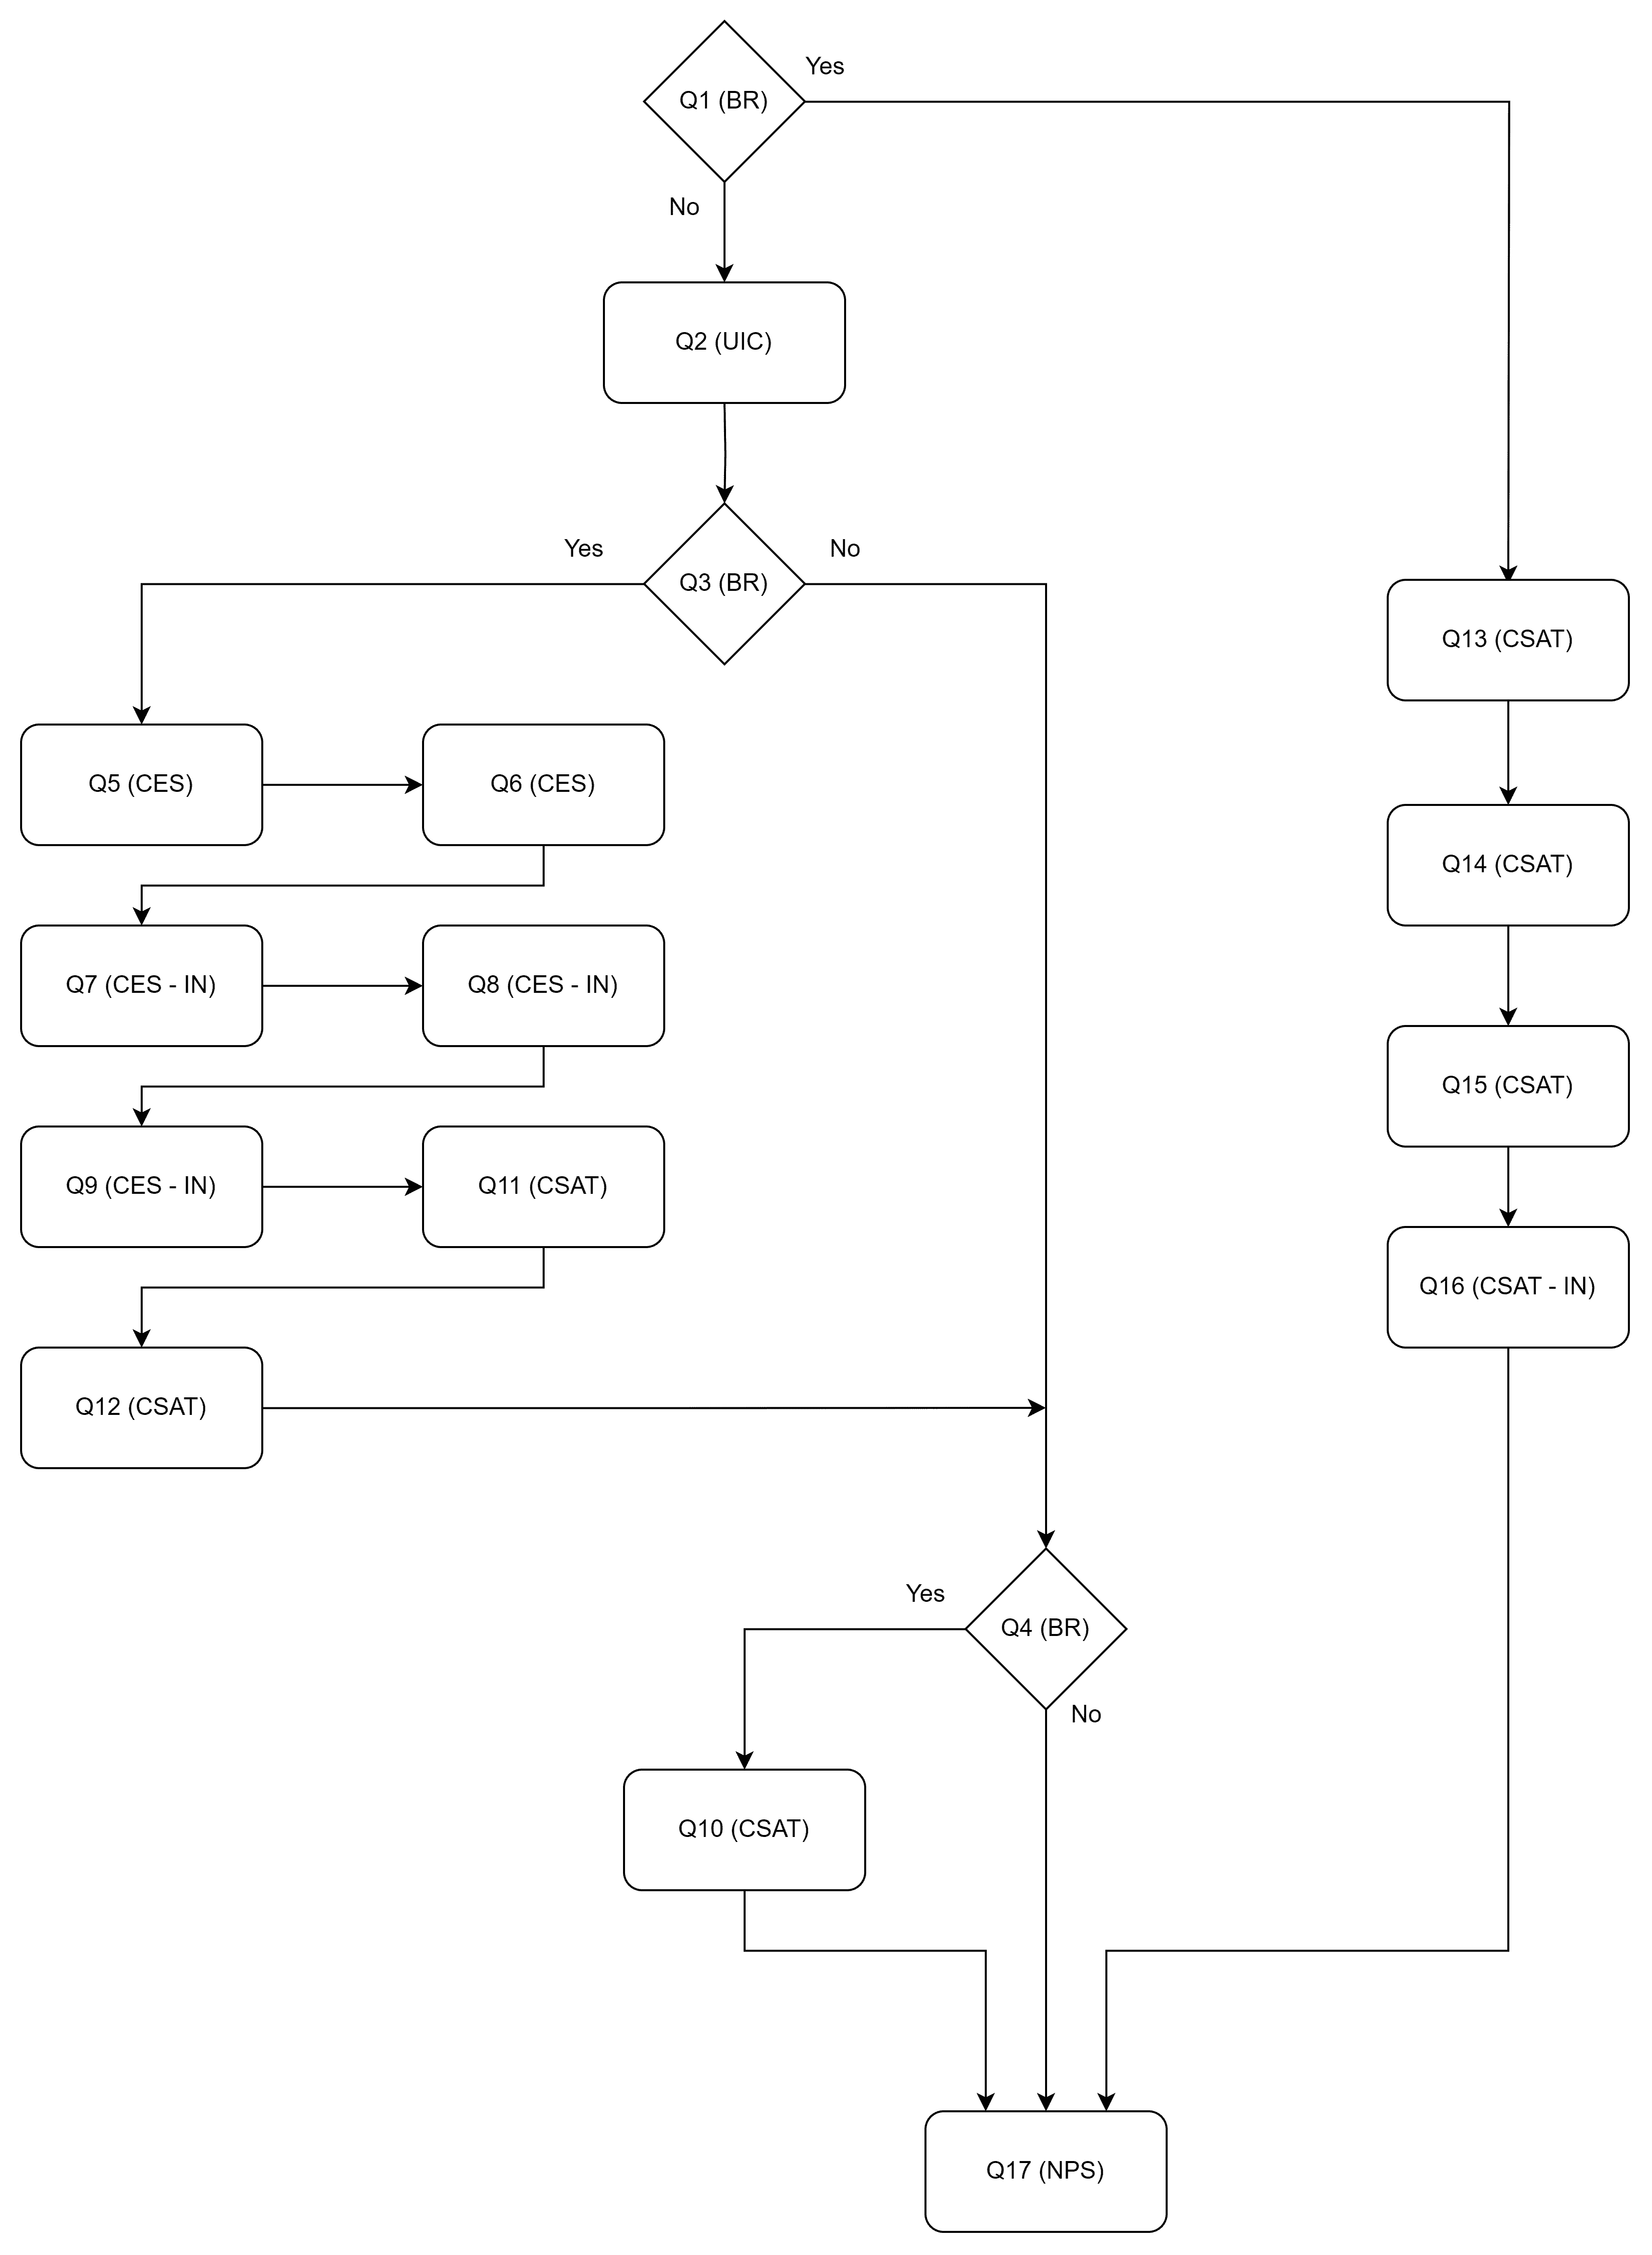
\includegraphics[width = \linewidth]{Content/Cơ sở lý thuyết/documents/Survey/images/surveyflow.png}
        \vspace{0.5cm}
        \caption{Trình tự câu hỏi trong bảng khảo sát}
        \label{fig:Trình tự câu hỏi trong bảng khảo sát}
    \end{figure}